%-----------------------------------------------------------------------
%                                                                 aa.tex
% AA vers. 9.3, LaTeX class for Astronomy & Astrophysics
% Demonstration file
%                                                       (c) EDP Sciences
%-----------------------------------------------------------------------
%
%\documentclass[referee]{aa}    % for a referee version
%\documentclass[onecolumn]{aa}  % for a paper on 1 column  
%\documentclass[longauth]{aa}   % for long lists of authors and/or affiliations. 
                                % This command displays the first eight authors on page 1
                                % and shift the whole list after the references.
                                % Ensure to separate each author with the \and command (see below)
%\documentclass[letter]{aa}     % for the letters
%\documentclass[bibyear]{aa}    % if the references are not structured
                                % according to the author-year natbib style

\documentclass{aa}  

\usepackage{graphicx}
\usepackage{txfonts}
\usepackage{lipsum}
\usepackage{subcaption}         % necessary for continued figures, example in section 3
                                % and appendix
\usepackage{lscape}             % to rotate a single page table, example in appendix.
                                % For landscape tables, see the longtable examples.
\usepackage{placeins}           % useful with \FloatBarrier, to keep 
                                % onecolumn floats from drifting to the next section
                                
%%%%%%%%%%%%%%%%%%%%%%%%%%%%%%%%%%%%%%%%
\usepackage[]{hyperref}
% To add links in your PDF file, use the package "hyperref"
% with options according to your LaTeX or PDFLaTeX drivers.
%%%%%%%%%%%%%%%%%%%%%%%%%%%%%%%%%%%%%%%%

\begin{document}

%%%%%%%%%%%%%%%%%%%%%%%%%%%%%%%%%%%%%%%%
% if you use custom commands in your title,
% ensure to check your title when submitting!
%%%%%%%%%%%%%%%%%%%%%%%%%%%%%%%%%%%%%%%%
\title{The extended stellar densities of the Sculptor and Ursa Minor dwarf galaxies}

\subtitle{Innate nature or tidal nurture?}

%%%%%%%%%%%%%%%%%%%%%%%%%%%%%%%%%%%%%%%% % Please separate each author with the \and command
%
% Please do not include ORCIDs next to author names.
% Only ORCIDs authenticated by individual authors in EDPS
% editorial system will be taken into account.
% ORCIDs included here will be removed.
%%%%%%%%%%%%%%%%%%%%%%%%%%%%%%%%%%%%%%%%

   \author{D. A. Boyea\inst{1}
        \and others
        }

   \institute{EDP Sciences, 91940, Les Ulis, France\\
             \email{danielaboyea@gmail.com}
             \thanks{Shows the usage of elements in the institute field}
            \and FSTT, 90000, Tanger, Morocco\\ }

   \date{Received December XX, 20XX}

% \abstract{}{}{}{}{}
% 5 {} token are mandatory
 
  \abstract
  % context heading (optional)
  % {} leave it empty if necessary  
   {Optional, leave empty if necessary.  The heading “Context” is used when needed to
give background information on the research conducted in the paper}
  % aims heading (mandatory)
   {Mandatory. The objectives of the paper are defined here.} 
  % methods heading (mandatory)
   {Mandatory. The methods of the investigation are outlined here}
  % results heading (mandatory)
   {Mandatory. The results are summarized here.}
  % conclusions heading (optional), leave it empty if necessary
   {Optional, leave empty if necessary.  “Conclusions” can be used to
explicit the general conclusions that can be drawn from the paper.}

   \keywords{giant planet formation --
                $\kappa$-mechanism --
                stability of gas spheres
               }

   \maketitle


%%%%%%%%%%%%%%%%%%%%%%%%%%%%%%%%%%%%%%%%%%%%%%%%%%%%%%%%%%%%%%
\section{Introduction}
\lipsum[1]
%%%%%%%%%%%%%%%%%%%%%%%%%%%%%%%%%%%%%%%%%%%%%%%%%%%%%%%%%%%%%%
\section{{\it Gaia} Data}

\begin{figure}
    \centering
    \includegraphics{figures/classical_dwarf_profiles.pdf}
    {\caption{The density profiles of classical dwarfs, using data from \citet{jensen+2024}.}}
    \label{fig:observed_density_profiles}
\end{figure}

\section{Methods}

\begin{figure}
    \centering
    \includegraphics{figures/scl_lmc_xyzr_orbits.pdf}
    \caption{
        Orbits of Sculptor with and without the LMC.
    }
    \label{fig:scl_orbits}
\end{figure}


\begin{figure}
    \centering
    \includegraphics{figures/umi_xyzr_orbits.pdf}
    \caption{
        Orbits of Ursa Minor
    }
    \label{fig:umi_orbits}
\end{figure}


\section{Results}

\subsection{Sculptor}

\begin{figure*}
    \centering
    \includegraphics{figures/scl_lmc_sim_images.png}
    \caption{Snapshots of Scl in the LMC and MW potential.}
    \label{fig:scl_sim_images}
\end{figure*}

\begin{figure}
    \centering
    \includegraphics{figures/scl_density_i_f.pdf}
    \caption{Simulated initial and final stellar density profiles for a tidal simulation of Scl in the MW+LMC potential} 
    \label{fig:scl_density_i_f}
\end{figure}


\subsection{Ursa Minor}
\begin{figure*}
    \centering
    \includegraphics{figures/umi_sim_images.png}
    \caption{Snapshots of UMi's tidal evolution in the MW potential}
    \label{fig:umi_sim_images}
\end{figure*}

\begin{figure}
    \centering
    \includegraphics{figures/umi_density_i_f.pdf}
    \caption{Similar to \ref{fig:scl_density_i_f} except for UMi.} 
\end{figure}


%%%%%%%%%%%%%%%%%%%%%%%%%%%%%%%%%%%%%%%%%%%%%%%%%%%%%%%%%%%%%%
\section{Conclusions}



%%%%%%%%%%%%%%%%%%%%%%%%%%%%%%%%%%%%%%%%%%%%%%%%%%%%%%%%%%%%%%
\begin{acknowledgements}
\end{acknowledgements}



\bibliographystyle{aa} % style aa.bst
\bibliography{paper} % your references Yourfile.bib


%\begin{appendix}
%
%\onecolumn
%\section{Wide tables and figures after an appendix title: recommended method}
%
%In the PDF output, \underline{floats should be placed
%under their own appendix}, not before the title, nor after the
%title of the next appendix. In short appendices, one-column floats
%\{figure*\} or \{table*\} will generate
%a blank page. To prevent this behaviour, we recommend to switch
%to \textbackslash onecolumn and set the [ht!] parameter 
%in your floats: please check the \LaTeX code of this appendix.\\
%
%In case you have a lot of floating objects for little text and the 
%\LaTeX engine moves the floats away from their context, the command
%\textbackslash FloatBarrier of the “placeins” package will empty the
%float buffer and place all stored floats in the continuity. If you still encounter problems with wide floats placement, just use the \textbackslash onecolumn
%environment throughout the appendices.
%
%
%\begin{figure*}[ht!]
%    \centering
%     \resizebox{12cm}{12cm}
%    {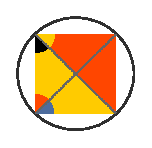
\includegraphics {figure.eps}}
%     \caption{A one-column \{figure*\}[ht!] after a section title.
%      If text follows like below, it is easier to finish the section in
%      \textbackslash onecolumn. If needed, you may revert to \textbackslash
%      twocolumn when reaching the next page.}
%      \label{fig5ap}
%\end{figure*}
%
%
%
%\end{appendix}
\end{document}
